\documentclass{article}

\usepackage[dutch]{babel}
\usepackage{epsfig}
\usepackage{verbatim}
\usepackage{amsmath}

\author{Peter van Dijk \& Elizabeth Schermerhorn}
\date{\today}
\title{Practicum 2 Betrouwbare communicatie}
\begin{document}
\maketitle
\newpage
\tableofcontents
\clearpage
\section{Packet Error Rate-metingen}
\subsection{Inleiding}
De Nordic RF24 is een radiozender en -ontvanger voor de 2.4GHz band. De RF24 heeft echter een aantal verschillende instellingen voor de kanalen, outputpower en datasnelheid. Het doel van dit onderzoek is bepalen wat de optimale instellingen zijn om de Packet Error Rate (PER) zo laag mogelijk te krijgen. Door middel van de volgende vergelijking wordt de Packet Error Rate berekend: 
\setlength{\parskip}{10pt plus 1pt minus 1pt}

$\frac {incorrect-ontvangen}{correct-ontvangen}$

	
 Eerst zal de probleemstelling besproken worden samen met vastgestelde hypothesen, vervolgens zal de methodologie aan bod komen en als laatste zullen de resultaten besproken en geanalyseerd worden. 

\subsection{Probleemstelling}
De onderzoeksvraag die hier beantwoord zal worden is: \textit{"Voor welke waarden voor de outputpower, transmissiesnelheid en frequentiekanaal is de PER het laagst."} Hierbij horen de volgende hypothesen: 
\begin{enumerate}
  \item Op het moment dat er meerdere mensen op hetzelfde frequentiekanaal zitten zal dit voor veel pakket verlies zorgen.
  \item Bij een hogere outputpower zal het pakketverlies kleiner zijn.
  \item Bij een hogere transmissiesnelheid zal er meer pakketverlies optreden. 
\end{enumerate}
In het volgende onderzoek zullen deze hypothesen getoetst worden.
\subsection{Methodologie}
Om deze hypothesen te toetsen moeten er metingen gedaan worden. Hier zijn verschillende zaken van belang. 
\begin{itemize}
	\item De gebruikte hardware
	\item De gebruikte software
	\item De instellingen/vastgestelde constanten
	\item De onderzoeksopstelling
\end{itemize}

%De gebruikte hardware
\subsubsection{De hardware}
De Hardware die gebruikt is bij de metingen is een Arduino UNO en een Nordic nRF24L01 draadloze transceiver.\\

%de gebruikte software
\subsubsection{De software}
Om de hardware te gebruiken wordt gebruik gemaakt van de opensourcesoftwarebibliotheek voor de Arduino, die te vinden is op: \begin{verbatim}http://maniacbug.github.io/RF24/ \end{verbatim} 
Met deze software kan de radio aangestuurd worden en kunnen pakketjes worden verzonden en ontvangen. De radio luistert en verstuurt pakketten over een bepaald kanaal. Het is van belang dat de radio's hetzelfde kanaal gebruiken, zodat ze met elkaar kunnen communiceren. De kanalen hebben een nummer van 0 tot en met 125.\\
\\
Om de metingen uit te voeren en onze hypotheses te testen is er gebruik gemaakt van \'{e}\'{e}n zender en \'{e}\'{e}n ontvanger. De zender gebruikt \texttt{sender.ino} en de ontvanger gebruikt \texttt{receiver.ino}. Deze programma's zijn te vinden in de appendix. De zender zend pakketjes met daarin het pakketnummer. De ontvanger begint met luisteren en onthoudt het nummer van het eerste pakketje dat hij heeft ontvangen. Vervolgens zal de ontvanger blijven luisteren totdat deze 1000 pakketten heeft ontvangen. Uit de inhoud van het laatste pakket kan worden opgemaakt hoeveel pakketten er verloren zijn gegaan voor de duizend die er ontvangen zijn. De PER wordt berekend met de formule:\\
\\
\indent	$(([laatste pakketnummer]-[eerste pakketnummer])/[aantal ontvangen pakketten])$\\
\\
In de software van de Sender en Receiver is gebruik gemaakt van de volgende drie methoden om de verschillende waarden aan te kunnen passen. 
\begin{itemize}
	\item setChannel(uint\char`_8 i) \\
	met 0 $\leq$ i $\leq$ 125
	\item setPALevel(PALevel level) \\
	met level $\in \{$  RF24\_PA\_MAX, RF24\_PA\_MIN, RF24\_PA\_LOW $\}$
	\item setDataRate(Rate rate) \\
	met rate $\in \{$ RF24\_1MBPS, RF24\_2MBPS$\}$
\end{itemize}
Door met deze drie methoden de waarden aan te passen verkrijgen we de gewilde meetresultaten. Deze zullen in sectie 1.4 besproken worden.

\subsubsection{De instellingen/vastgestelde constanten}
Om deze metingen bruikbaar te houden moeten er een paar constanten gedefinieerd worden.
\begin{itemize}
	\item De grootte van de payload
	\item Het aantal te versturen berichten
\end{itemize}
Het aantal keer dat er een pakket opnieuw verstuurd wordt is niet van belang in deze implementatie omdat het zo ge\"{i}mplementeerd is dat het aantal ontvangen berichten wordt bijgehouden en het aantal verzonden berichten wordt bijgehouden. 
Voor de grootte van de payload is er gekozen voor de grootst mogelijke waarde die deze kan aannemen, namelijk 255 bytes. Deze waarde is gekozen omdat de onderzoeksvraag is wanneer is de radio communicatie het meest betrouwbaar en dit moet getest worden voor re\"{e}le waarden. 
Het aantal te versturen berichten is op 1000 gezet. Hier is voor gekozen vanwege het idee omdat meer waarden betekent nauwkeurigere resultaten.
\\
\\
De meetopstelling bestaat uit twee radio's welke 270cm uit elkaar geplaatst zijn. Om de resultaten consistent te houden moet bij elke meting deze afstand aangehouden worden. 
Verder worden bericht niet opnieuw verzonden als er geen acknowledgement volgt, want dit betekent pakket verlies en dat moet gemeten worden. 

\subsection{Resultaten en analyse}
Hier zullen de resultaten weergegeven en geanalyseerd worden. \\*
  De constanten zoals ze standaard gebruikt zullen worden. Als ze gewijzigd worden voor de test dan wordt dit aangegeven. 
  \begin{itemize}
  	\item afstand tussen radio's: 270 cm
  	\item Geen hertransmissie van pakketten
  	\item payload: 255 bytes
  	\item channel: 125
  \end{itemize}
  
\subsubsection{Metingen en resultaten}
Tijdens de metingen waren er geen andere radio's aan het sturen, waardoor de radio's geen last van interferentie hadden.\\
\\
    \begin{tabular}{ | l | l | l | p{5cm} |}
    \hline
    Instellingen 				& PER 		& gemiddelde PER\\ \hline
    outputpower: MAX 			& 1/1000 	& 2/3000		\\
    transmissiesnelheid: 2MBps 	& 1/1000 	& 				\\
    delay: 25 ms 				& 0/1000	&  				\\ \hline
    \end{tabular}\\
\\
\\
    \begin{tabular}{ | l | l | l | p{5cm} |}
    \hline
    Instellingen				& PER 		& gemiddelde PER\\ \hline
    outputpower: MAX 			& 0/1000 	& 0/3000		\\
    transmissiesnelheid: 2MBps 	& 0/1000 	&  				\\
    delay: 50 ms 				& 0/1000	&  				\\ \hline
    \end{tabular}\\
\\
\\
    \begin{tabular}{ | l | l | l | p{5cm} |}
    \hline
    Instellingen 				& PER 		& gemiddelde PER\\ \hline
    outputpower: MAX 			& 0/1000 	& 0/3000		\\
    transmissiesnelheid: 1MBps 	& 0/1000 	&  				\\
    delay: 50 ms 				& 0/1000	&  				\\ \hline
    \end{tabular}\\
\\
\\
    \begin{tabular}{ | l | l | l | p{5cm} |}
    \hline
    Instellingen				& PER 		& gemiddelde PER\\ \hline
    outputpower: MIN 			& 85/1000 	& 1273/3000		\\ 
    transmissiesnelheid: 2MBps 	& 669/1000  &  				\\ 
    delay: 50 ms 				& 519/1000 	&  				\\ \hline
    \end{tabular}\\
\\
\\
    \begin{tabular}{ | l | l | l | p{5cm} |}
    \hline
    Instellingen				& PER 		& gemiddelde PER\\ \hline
    outputpower: LOW 			& 0/1000 	& 8/3000		\\ 
    transmissiesnelheid: 2MBps 	& 2/1000 	&   			\\ 
    delay: 50 ms 				& 6/1000 	&  				\\ \hline
    \end{tabular}\\
\\
\\
    \begin{tabular}{ | l | l | l | p{5cm} |}
    \hline
    Instellingen				& PER 		& gemiddelde PER\\ \hline
    outputpower: MAX 			& 0/1000 	&  0/3000		\\ 
    transmissiesnelheid: 2MBps 	& 0/1000 	&   			\\ 
    delay: 50 ms 				& 0/1000 	&				\\ 
    channel: 0 					&  			&  				\\ \hline
    \end{tabular}\\
\\
\\
    \begin{tabular}{ | l | l | l | p{5cm} |}
    \hline
    Instellingen				& PER 		& gemiddelde PER\\ \hline
    outputpower: MAX 			& 0/1000 	& 1/3000		\\ 
    transmissiesnelheid: 2MBps 	& 1/1000 	&  				\\ 
    delay: 50 ms 				& 0/1000 	&  				\\ 
    channel: 64 				&  			&				\\ \hline
    \end{tabular}\\
\\
\\
Verder zijn er nog enkele kleinere tests uitgevoerd op een netwerk met interferentie. Dit leverde de volgende resultaten:\\
\\
\begin{tabular}{ | l | l | l | p{5cm} |}
    \hline
    Instellingen				& PER 		& gemiddelde PER\\ \hline
    outputpower: MAX 			& 47/300 	& 433/3000		\\ 
    transmissiesnelheid: 2MBps 	& 77/300 	&  				\\ 
    delay: 50 ms 				& 9/300 	&  				\\ \hline
    \end{tabular}\\
\\
\\
Om het resultaat nauwkeuriger en accurater te kunnen weergeven is ervoor gekozen om alle tests in drievoud uit te voeren zodat vreemde gebeurtenissen opgemerkt worden. Een voorbeeld is een error rate $>$ 1. Tussen deze resultaten is de instelling HIGH voor outputpower niet weergegeven, aangezien deze voor de gebruikte versie van de radio niet een mogelijke waarde was.

\subsection{Conclusie}
Als er naar de gevonden waarden gekeken wordt, is de PER onacceptabel wanneer de outputpower op MIN staat. Een gemiddelde PER van 1273/3000 pakketten zorgt op den duur voor veel hertransmissies dus veel vertraging op het netwerk. Dit is een situatie die niet gewenst is. Wanneer naar de overige instellingen gekeken wordt en de daarbij behorende gemiddelde PER dan zijn ze perfect of een PER $<$ 0.01. Hier moet bij vermeld worden dat op het moment dat er meer interferentie is op het netwerk de PER omhoog schiet op het netwerk. Op dat moment is het kiezen van een ongebruikt frequentiekanaal van belang. Dit experiment heeft plaats gevonden in een interferentievrije ruimte.\\
\\
De onderzoeksvraag is: \textit{"Voor welke waarden voor de outputpower, transmissiesnelheid en frequentiekanaal is de PER het laagst."} Het antwoord dat hierbij hoort is dat voor elke waarde van de transmissiesnelheid en het frequentiekanaal de PER niet boven de 0.01 uit komt. Dit geldt echter niet voor de outputpower; op het moment dat de outputpower op minimaal gezet wordt bedraagt de gemiddelde PER 1273/3000. Hieruit kan geconcludeerd worden dat de outputpower tenminste op laag of maximaal gezet moet worden om de PER tot een minimum te beperken. 

\newpage

\clearpage
\section{Betrouwbare end-to-end-communicatie}

\subsection{Inleiding}
In het vorige experiment is de betrouwbaarheid van een singlehop-netwerk onderzocht. Nu kan de betrouwbaarheid van een multihop-netwerk getoetst worden en kunnen de waarden vergeleken worden om te bepalen welk netwerk betrouwbaarder is. 
\subsection{Probleemstelling}

De probleemstelling waarvan uit zal worden gegaan is \textit{"Is het mogelijk een betrouwbaar end-to-end multihop-connectie op te zetten?"}. De hypothese is dat dit mogelijk is in combinatie met :
\\
\begin{itemize}
	\item MIN zal het slechtst presteren en MAX het beste(transmissie sterkten)
	\item alternating bit protocol(ABP)
	Met deze drie aspecten verwerkt in de implementatie zou het multihop-netwerk moeten werken. 
\end{itemize}
\subsection{Protocol}
Het protocol wat veelal gebruikt wordt in deze implementatie is het ABP. Dit protocol houdt twee zaken in:
\\
\begin{itemize}
	\item hertransmissies sturen
	\item kijken of er iets binnenkomt
\end{itemize}
Het ABP zorgt ervoor dat wanneer er geen acknowledgement ontvangen wordt er een hertransmissie gestuurd wordt. Door een bit op 0 of 1 te zetten kan er gekeken worden of er nieuwe data ontvangen wordt of niet. Dit is de globale werking van het protocol. Dit protocol is gebruikt in de implementatie van het multihop-netwerk, veelal op dezelfde manier maar dit zal toegelicht worden. 
\\ 
In de implementatie komt dit protocol terug in alle nodes.
Alle nodes moeten weten of er berichten binnen komen. Om dit te registreren is er gekozen voor het ABP.\\

De zender verstuurt de berichten en wacht totdat er een acknowledgement terugkomt voordat een nieuw bericht wordt verstuurd. Op het moment dat er een time-out plaatsvind zal er een hertransmissie plaatsvinden. Op het moment dat er een bericht binnenkomt dan zal dit geregistreerd worden en zal dit bericht verder worden afgehandeld.

\begin{figure}
\centering 
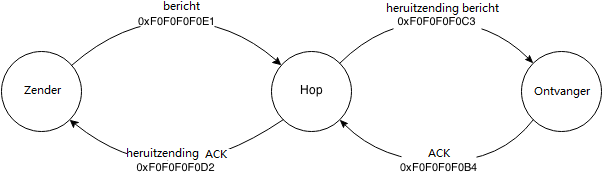
\epsfig{file=img/hop.png,width=\linewidth} 
\caption{Opstelling van het netwerk}
\label{fig:hop} %always place your label after your caption!
\end{figure}

\subsection{Methodologie}
Om de onderzoeksvraag te kunnen beantwoorden is er een meetopstelling nodig. De meetopstelling is weergegeven in Figuur \ref{fig:hop} met een Sendernode, een Hopnode en een Receivernode.
De namen geven het al aan, de Sendernode stuurt de berichten (en wacht op bevestiging), de Hopnode stuurt de berichten door en de Receivernode ontvangt de berichten (en bevestigd de ontvangst).  

\subsubsection{De software}

De software die gebruikt is voor dit experiment is grotendeels hetzelfde als het voorbeeld pingpair dat wordt meegeleverd bij de RF24 library voor de Arduino. In deze implementatie zijn slechts de adressen van de pipes gewijzigd naar de vier die te zien zijn in Figuur \ref{fig:hop} en is de pakketgrootte veranderd naar 255 bytes. 

De Hopnode luistert naar de Sendernode en Receivernode en stuurt berichten van de Sendernode door naar de Receivernode en andersom. In de implementatie is ervoor gezorgd dat er hertransmissies gestuurd kunnen worden als er een time-out optreed.
Er is gebruik gemaakt van een aantal constanten, namelijk:

\begin{itemize}
	\item payload = 255 bytes
	\item hertransmissies : 15
	\item delay: 50ms
	\item transmissiesnelheid: 2MBps
\end{itemize}  
Deze constanten zullen tijdens het testen niet worden veranderd.

\subsubsection{De hardware}

Deze bestaat uit drie identieke nodes. Deze nodes zijn allemaal voorzien van een radio waarmee ze de berichten kunnen ontvangen en versturen. De nodes zijn in een lijn geplaatst met een meter afstand tussen Sender en Hop en tussen Hop en Receiver. De experimenten zijn uitgevoerd in een netwerk waar nog meer radio\'s aan het sturen zijn.
 
\subsection{Resultaten en analyse}

Om de resultaten te verkrijgen die gewenst zijn worden er telkens andere waarden gebruikt voor de transmissie sterkte.
De transmissiesterkte geldt voor alle drie de nodes(zender, hop en ontvanger). De drie waarden die hiervoor gebruikt zijn:

\begin{itemize}
	\item RF24\_PA\_MIN
	\item RF24\_PA\_LOW
	\item RF24\_PA\_MAX
\end{itemize}
De waarden die gevonden zijn bij de volgende instellingen volgen hieronder.
\\
\\
    \begin{tabular}{ | l | l | l | p{5cm} |}
    \hline
    Instellingen 				& PER 		& gemiddelde PER\\ \hline
    outputpower: MIN 			& 1/1000 	& 25/3000		\\
    							& 17/1000 	& 				\\
   								& 7/1000	&  				\\ \hline
    \end{tabular}\\
\\
\\
    \begin{tabular}{ | l | l | l | p{5cm} |}
    \hline
    Instellingen 				& PER 		& gemiddelde PER\\ \hline
    outputpower: LOW 			& 0/1000 	& 2/3000		\\
    							& 1/1000 	& 				\\
   								& 1/1000	&  				\\ \hline
    \end{tabular}\\
\\
\\
    \begin{tabular}{ | l | l | l | p{5cm} |}
    \hline
    Instellingen 				& PER 		& gemiddelde PER\\ \hline
    outputpower: MAX 			& 0/1000 	& 1/3000		\\
    							& 0/1000 	& 				\\
   								& 1/1000	&  				\\ \hline
    \end{tabular}\\
\\
In de bovenstaande drie grafieken staan de PER samen met de transmissie sterkte waarmee de pakketjes verstuurd zijn. Er moet rekening gehouden worden met de omgeving waarin deze experimenten zijn uitgevoerd. 

\subsection{Conclusie}

De hypothese die gesteld werd: \textit{"Is het mogelijk een betrouwbaar end-to-end multihop-connectie op te zetten?"}.
Deze hypothese wordt nu gestaafd door de resultaten die verkregen zijn door de experimenten uit te voeren met veranderende transmissie sterktes. 
Uit de grafieken bij 2.5 kan opgemaakt worden dat een multi-hop verbinding, welke op deze manier ge\"{i}mplementeerd is, een redelijke implementatie geeft met een lage error rate. Zoals verwacht in de hypothese is zenden op minimum de slechtst scorende, maar zolang je hertransmissies hebt is dit een degelijke implementatie. 
De hertransmissies komen voort uit het ge\"{i}mplementeerde alternating bit protocol. Door het ABP en de beste transmissie sterkte te kiezen is er een stabiel netwerk opgezet wat in het dagelijks leven toegepast kan worden. 
\clearpage




\appendix
\section{De radio en de RF24-library}
\subsection{Eigenschappen van de RF24}
In dit onderzoek wordt gebruik gemaakt van de rf24 radio. Deze radio heeft de volgende eigenschappen:
	\begin{itemize}	
	\item\textbf{Frequentieband: }2.4000-2.4835 GHz
	\item\textbf{Datasnelheid: }1 of 2 Mb/s
	\item\textbf{Aantal kanalen: }126 RF-kanalen
	\item\textbf{Modulatietechniek: }Gaussian Frequency Shift Key(GFSK)
	\end{itemize}
	
\subsection{Energieverbruik}	
De radio het volgende energieverbruik in verschillende modi:\\
\\	
\begin{tabular}{|l|l|}
\hline
\textbf{Energiemodus}  & \textbf{Energieverbruik in Amp\`ere}     \\
\hline
Standby-I   & 22 $\mu$A    	\\
Standby-II  & 320 $\mu$A	\\
Power down  & 900 nA \\ \hline
\end{tabular}\\
\\
\\
\begin{tabular}{|l|l|}
\hline
\textbf{Zendmodus}  & \textbf{Energieverbruik in Amp\`ere}     \\
\hline
0 dBm  	& 11.3 mA	\\
-6 dBm 	& 9 mA    	\\
-12 dBm & 7.5 mA  	\\
-8 dBm 	& 7 mA		\\ \hline
\end{tabular}\\
\\
\\
\begin{tabular}{|l|l|}
\hline
\textbf{Ontvangstmodus}  & \textbf{Energieverbruik in Amp\`ere}     \\
\hline
2 Mbps  & 12.3 mA    \\
1Mbps	& 11.8 mA    \\ \hline 
\end{tabular}\\
\\

\subsection{Enhanced ShockBurst}

Een belangrijk aspect van de RF24 radio is Enhanced ShockBurst. Dit is een pakketgerichte datalinklayer protocol.
Belangrijke functies van Enhanched ShockBurst zijn:
\begin{itemize}
	\item Automatische pakket samenvoeging
	\item 6 data pipe multiceivers
	\item pakket afhandeling
\end{itemize}
Het formaat van het datapakket bestaat uit verschillende delen, het adres, pakket identificatie, geen acknowledgement bits en CRC. De velden hebben de volgende functies:
\\
\\
\begin{tabular}{ | l | l |}
    \hline
    Data veld					& Functie	\\ \hline
    Adres						& Het adres van de ontvanger	\\ \hline
    Pakket identificatie		& Om te achterhalen of het pakket een \\
    							& hertransmissie is.\\\hline
    geen acknowledgement bit	& Als deze bit gezet is mag het pakket niet\\
    							& automatisch erkend worden.	\\ \hline
    CRC							& Error detectie mechanisme voor het pakket			\\ \hline
    \end{tabular}
    
\subsubsection{Automatische hertransmissie}

Enhanced Shockburst heeft als eigenschap automatisch pakketvalidatie. In ontvangstmodus zoekt de RF24 constant naar valide adressen welke gegeven zijn in RX\_ADDR registers. Op het moment dat een valide adres gedetecteerd wordt, zal Enhanced Shockburst het pakket gelijk valideren. Enhanced Shockburst is voorzien van een ART(Automatic Retransmission) functie. Door deze functie is Enhanced Shockburst in staat een pakket uit zichzelf opnieuw te versturen als er geen acknowledgement wordt ontvangen. Er zijn drie redenen waarom de ART functie stopt met het luisteren na het versturen van een pakket. De ART stopt met luisteren na:
\begin{itemize}
	\item Auto retransmit delay(ARD) is verlopen
	\item Geen gematcht adres gevonden binnen 250$\mu$ s
	\item Nadat er een pakket ontvangen is
\end{itemize}
De radio is niet in staat om te broadcasten maar om deze functionaliteit te gebruiken moet er gebruik gemaakt worden van een multiceiver. 

\subsection{Adressering}
De adressen van een multiceiver moeten altijd sterk op elkaar lijken, alleen de least significant byte moet anders zijn. De volgende 4 adressen volgen uit dit principe:

\begin{itemize}
	\item  F0F0A
	\item  F0F0B
	\item  F0F0C
	\item  F0F0D
\end{itemize}
Doordat de Least significant byte anders is zijn dit vier geldige adressen.

\subsection{Functies}

Met de volgende functies worden waarden van de RF24 radio ingesteld:
\\
\begin{tabular}{ | l | l | p{5cm} |}
    \hline
    Functie				& Methode	\\ \hline
    Kanaal instellen	& void RF24::setChannel	(uint8\_t channel) 	\\ 
    Zendvermogen 		& void 	setPALevel (rf24\_pa\_dbm\_e level)	\\ 
    Aantal pogingen van ART instellen& void RF24::setRetries (uint8\_t delay, uint8\_t count )\\ 
    Adres van de zender instellen 	 & void	openWritingPipe (uint64\_t address)	\\
    Adres van de ontvanger instellen & void	openReadingPipe (uint8\_t number, uint64\_t address) \\ \hline
    \end{tabular}\\


\section{Code Sender}
\verbatiminput{./Sender/Sender.ino}

\section{Code Receiver}
\verbatiminput{./receiver/receiver.ino}

\section{Code Hop}
\verbatiminput{./Hopnetwerk/Hop/hop.ino}
\end{document}